\documentclass[12pt,a4paper]{article}
\usepackage[utf8]{inputenc}
\usepackage[turkish]{babel}
\usepackage{amsmath}
\usepackage{amsfonts}
\usepackage{amssymb}
\usepackage{graphicx}
\usepackage{float}
\usepackage{geometry}
\geometry{margin=2.5cm}

\title{DENEY 2: GLİSERİNİN VİSKOZİTE KATSAYISI}
\author{Ad Soyad \\ Öğrenci No: \\ Grup No: }
\date{\today}

\begin{document}

\maketitle

\section{Deneyin Amacı}
Stokes Yasası kullanarak herhangi bir sıvının viskozite katsayısının ölçülmesi.

\section{Teori}
Stokes Yasası'na göre, viskoz bir sıvı içinde hareket eden küre üzerinde sürtünme kuvveti etkir:

\begin{equation}
F = 6\pi\eta rv
\end{equation}

Terminal hız için denge denklemi:
\begin{equation}
\eta = \frac{2gr^2(\rho_{küre} - \rho_{sıvı})}{9v}
\end{equation}

\section{Deney Düzeneği}
\begin{itemize}
    \item Gliserin
    \item 100ml ölçülü silindir
    \item Termometre
    \item 5 farklı yarıçapda çelik bilye
    \item Kronometre
\end{itemize}

\section{Ölçümler ve Sonuçlar}

\subsection{Fiziksel Sabitler}
\begin{itemize}
    \item Çelik bilyenin kütle yoğunluğu: $\rho_{çelik} = 7850$ kg/m³
    \item Gliserinin kütle yoğunluğu: $\rho_{gliserin} = 1260$ kg/m³
    \item Yerçekimi ivmesi: $g = 9.81$ m/s²
    \item A-B arası mesafe: $L = $ \ldots m
    \item Gliserin sıcaklığı: $T = $ \ldots °C
\end{itemize}

\subsection{Ölçüm Tablosu}
\begin{table}[H]
\centering
\begin{tabular}{|c|c|c|c|c|c|c|}
\hline
Bilye & Çap (mm) & Yarıçap (mm) & Düşme Zamanı (s) & Terminal Hız (m/s) & Viskozite Katsayısı \\
\hline
1 & & & & & \\
2 & & & & & \\
3 & & & & & \\
4 & & & & & \\
5 & & & & & \\
\hline
\end{tabular}
\caption{Deneysel ölçümler}
\end{table}

\subsection{Grafikler}
\begin{figure}[H]
\centering
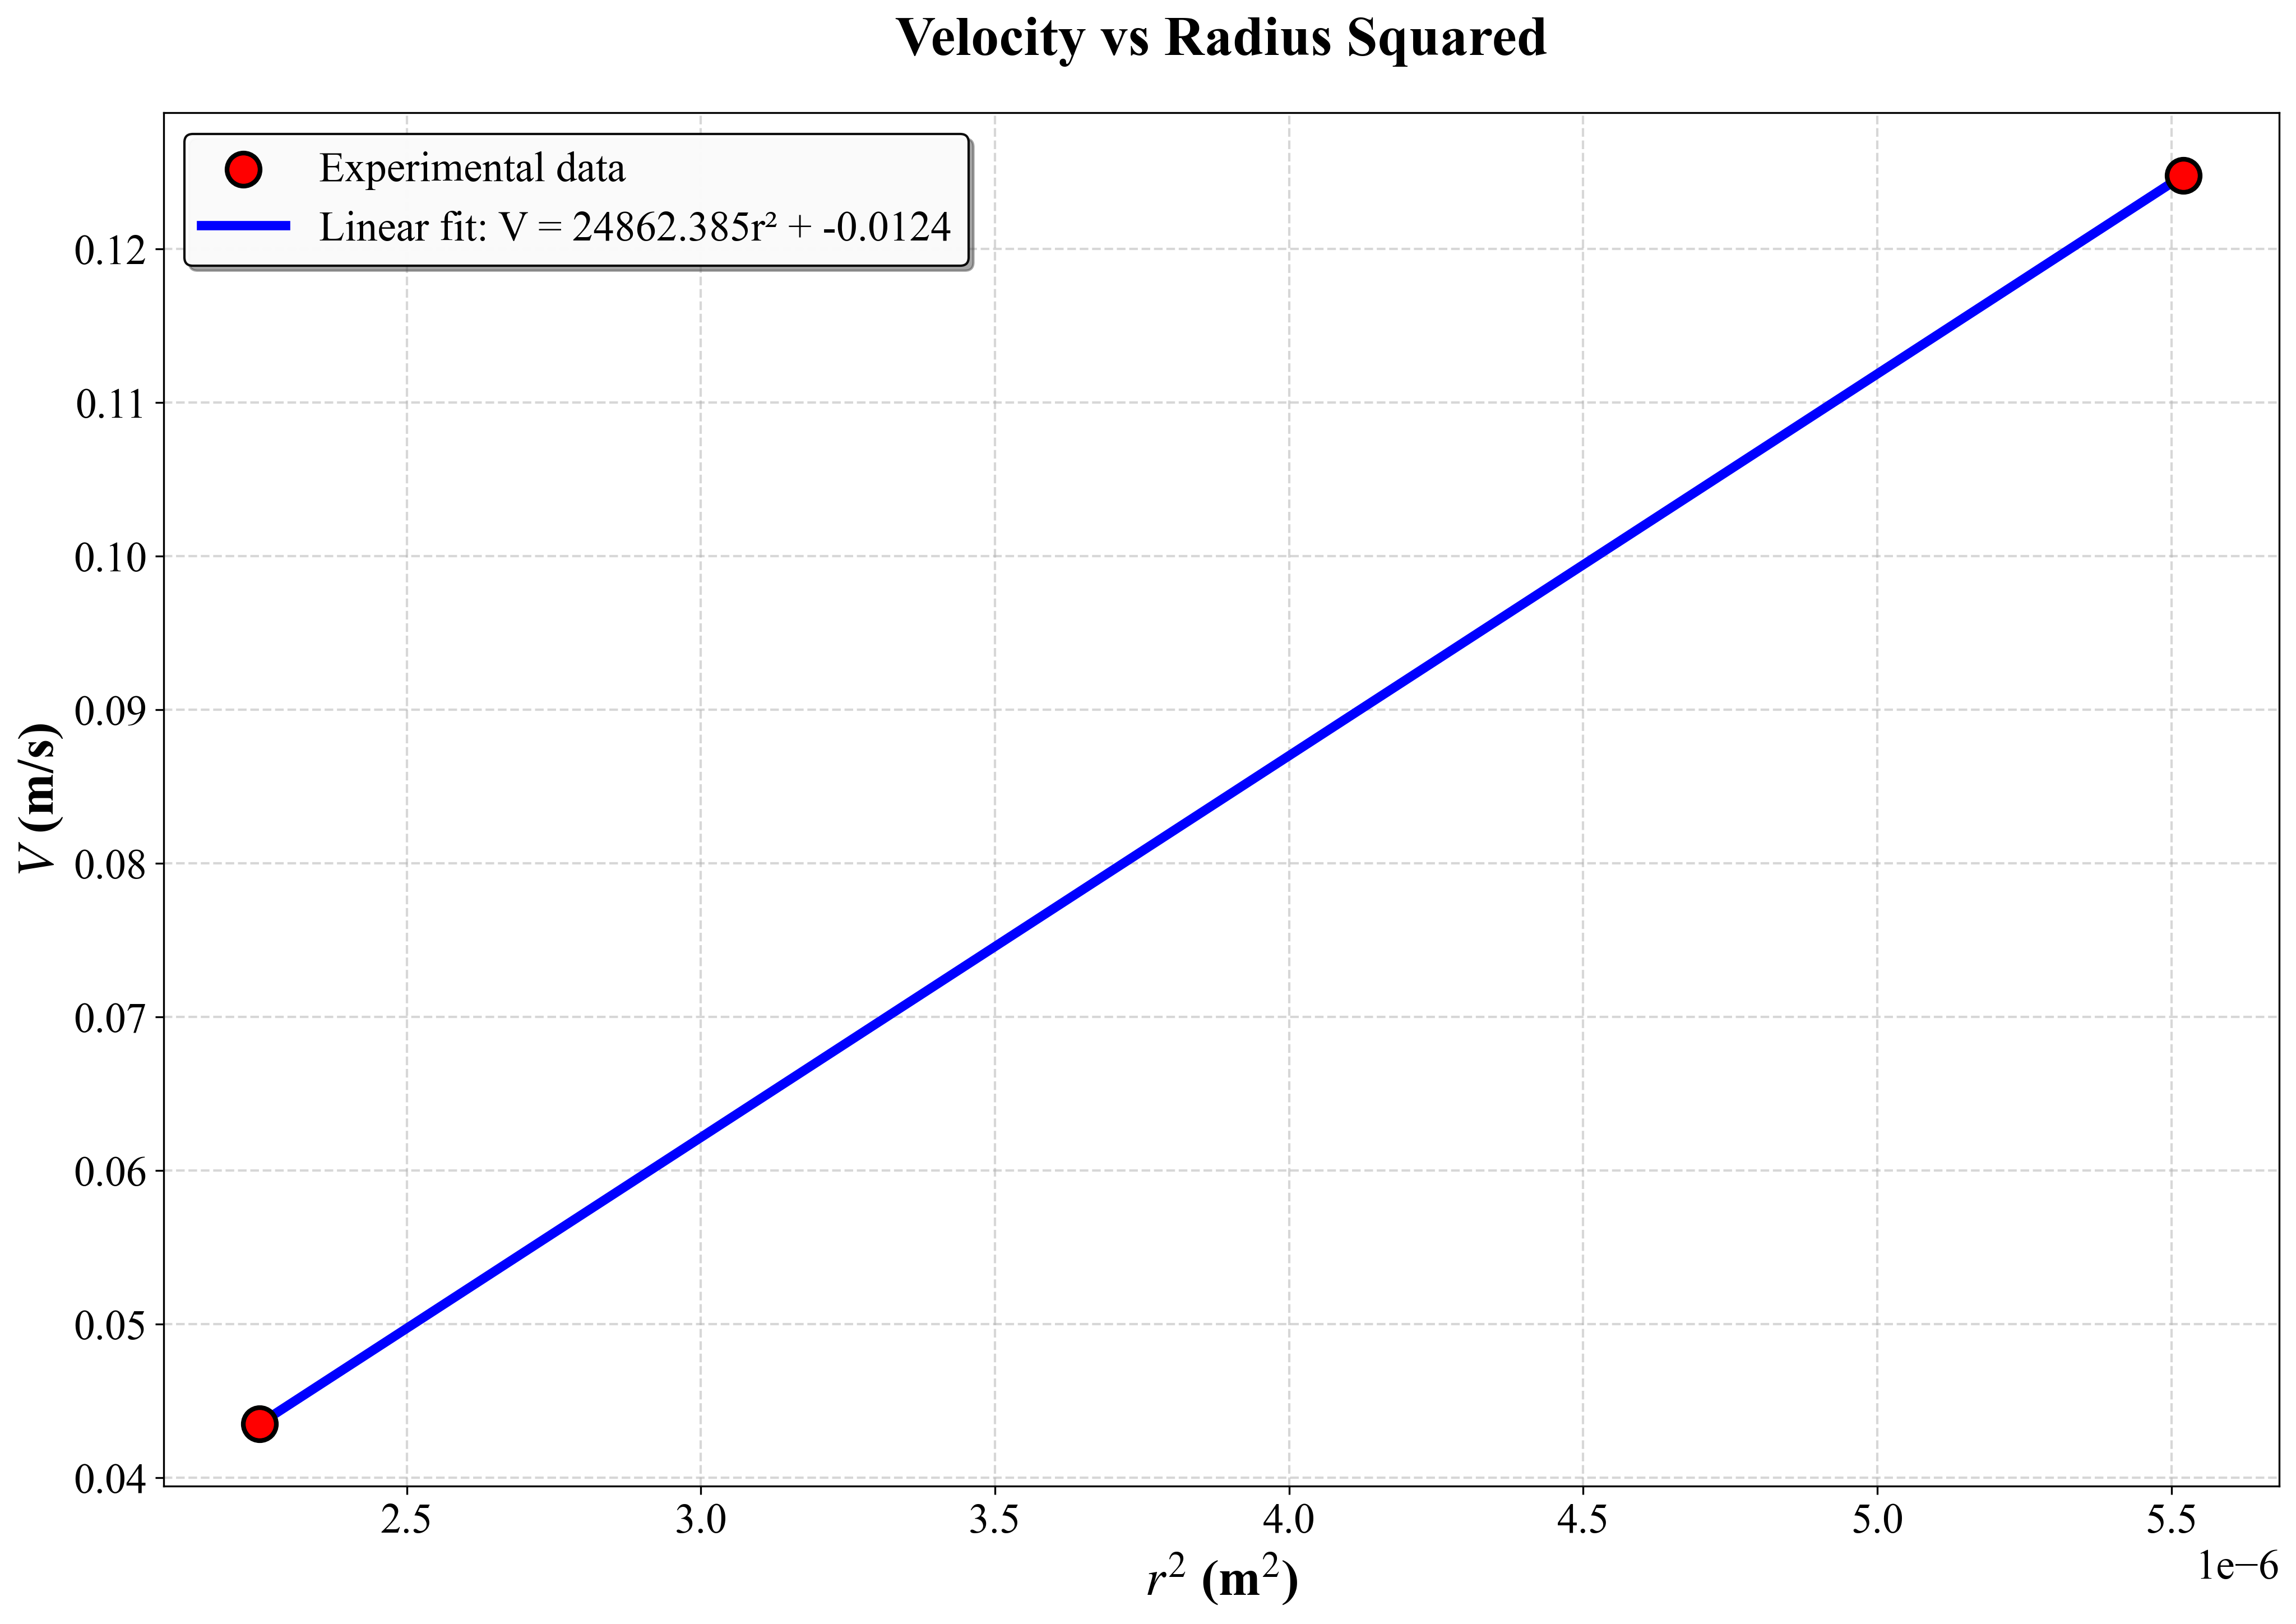
\includegraphics[width=0.8\textwidth]{velocity_vs_radius_squared.png}
\caption{Hız - Yarıçap² grafiği}
\end{figure}

\begin{figure}[H]
\centering
\includegraphics[width=0.8\textwidth]{graphs/viscosity_analysis.png}
\caption{Viskozite analizi}
\end{figure}

\section{Hata Analizi}
% Hata hesaplamaları ve standart sapma

\section{Sonuçlar ve Değerlendirme}
% Teorik değerlerle karşılaştırma ve yorumlar

\end{document}
